\chapter{Results}
\label{ch:results}

\begin{figure}
\centering
 \subtop[Final Result]
 {
  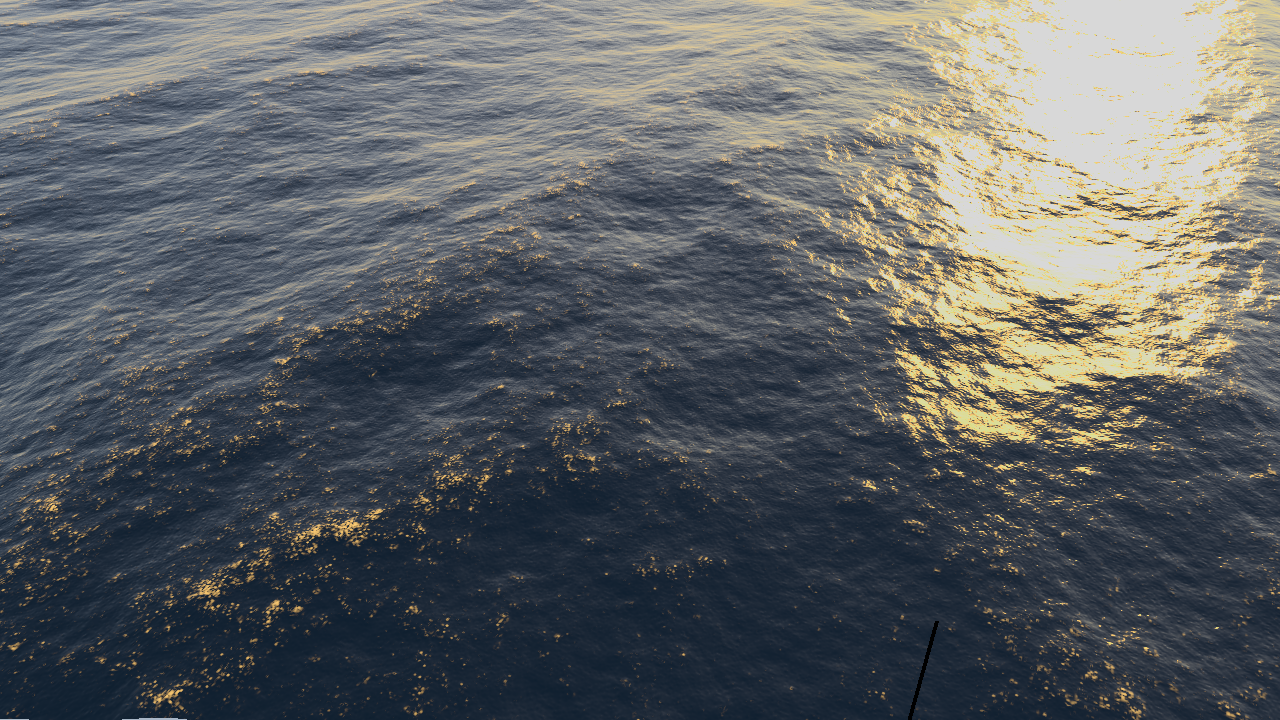
\includegraphics[width=\textwidth]{figures/31-07-2017_10-47-08_complete.png}
	%\label{fig:max1981:1}
 }
 \subtop[Ross BRDF Contribution]
 {
  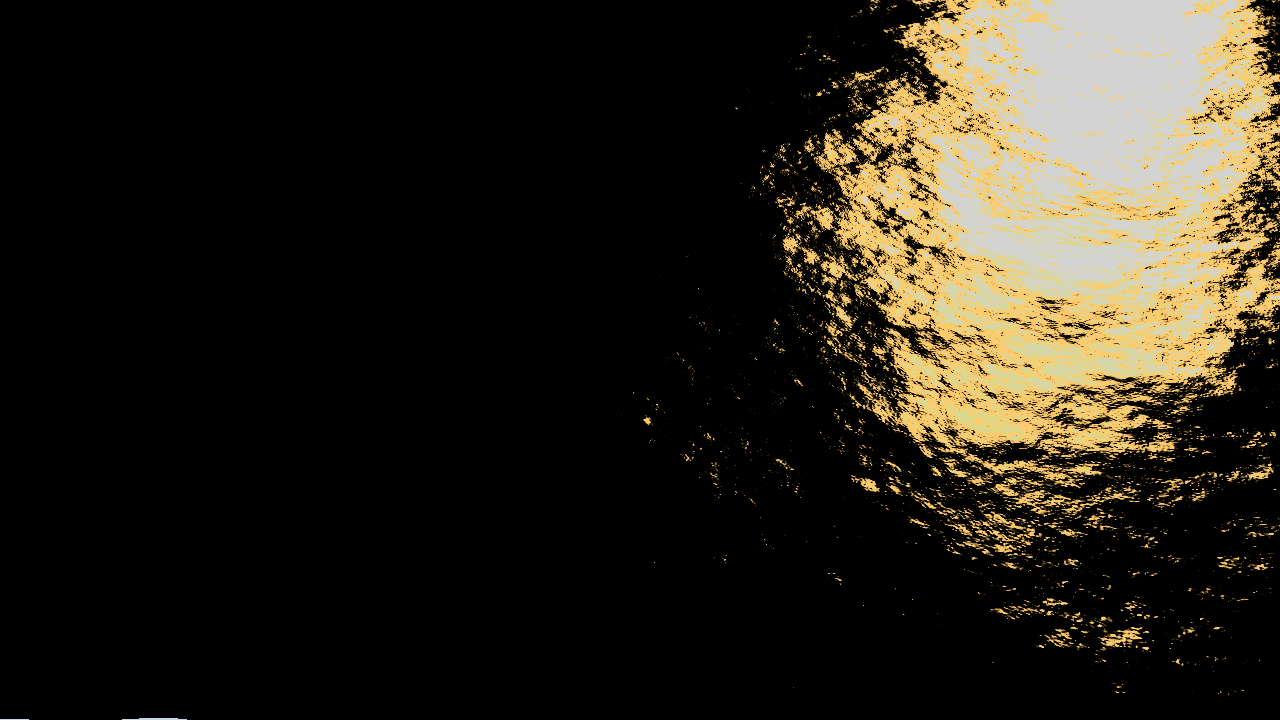
\includegraphics[width=0.45\textwidth]{figures/31-07-2017_10-47-08_ross.png}
	%\label{fig:max1981:2}
 }
 \hfill
 \subtop[Sea Contribution]
 {
  
\includegraphics[width=0.45\textwidth]{figures/31-07-2017_10-47-08_sea.png}
	%\label{fig:max1981:3}
 }
  \subtop[Sky Contribution]
 {
  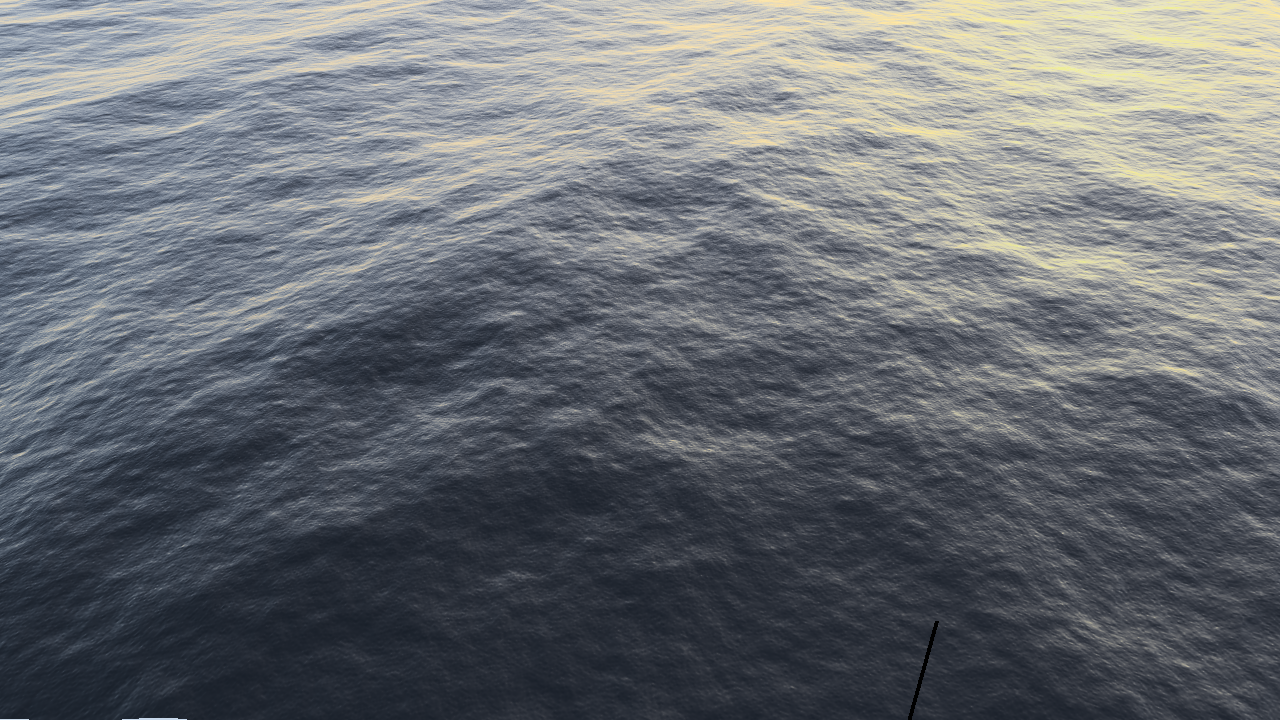
\includegraphics[width=0.45\textwidth]{figures/31-07-2017_10-47-08_sky.png}
	%\label{fig:max1981:4}
 }
 \hfill
 \subtop[Whitecaps Contribution]
 {
  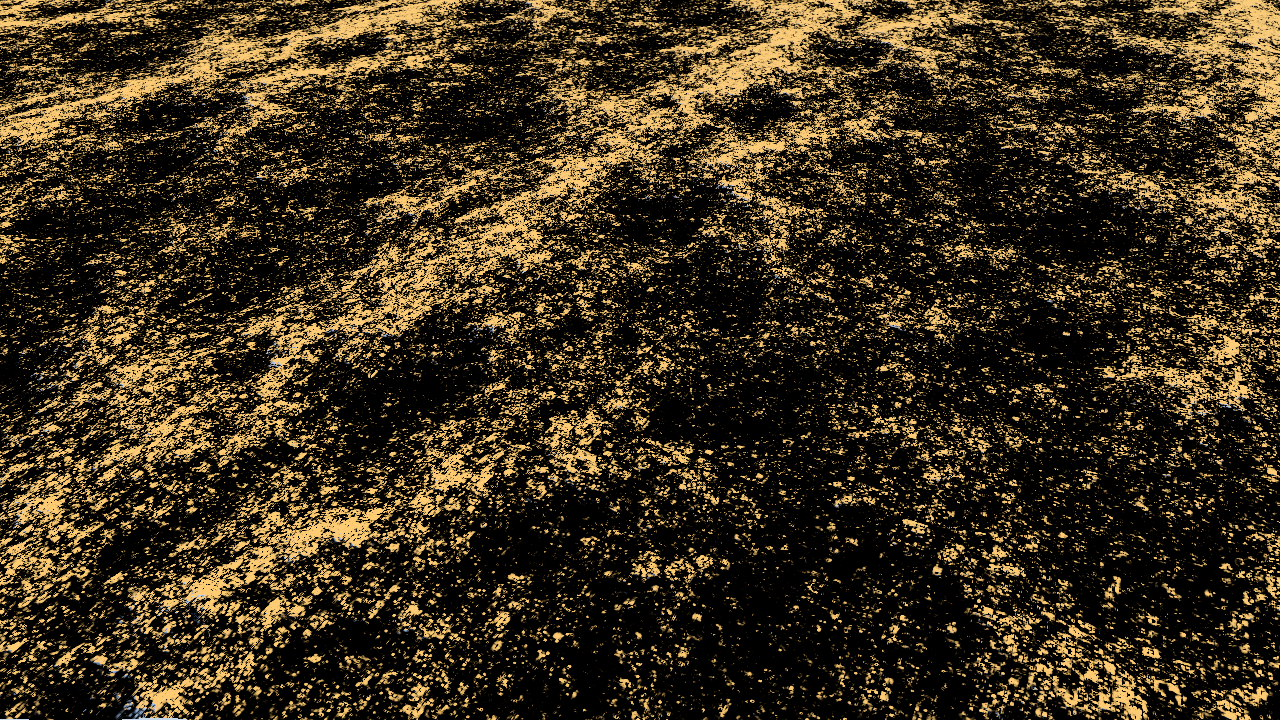
\includegraphics[width=0.45\textwidth]{figures/31-07-2017_10-47-08_whitecaps.png}
	%\label{fig:max1981:4}
 }
\caption{
%\subcaptionref{fig:max1981:1}~Still water near sunset.
%\subcaptionref{fig:max1981:2} One reflection from waves.
%\subcaptionref{fig:max1981:3} Two reflections from waves.
%\subcaptionref{fig:max1981:4} Early afternoon, two reflections from waves.
}
\label{fig:results}
\end{figure}

\section{Performance}

Simple \InvFourierTransform vs \InvFourierTransform of two hermitian spectra
Pattern synthesis at full resolution for all datasets
Pattern synthesis with our multi-resolution approach

\section{Visual Fidelity}

Images of all partial terms involved in ocean lighting (specular by sun,
reflection of sky, refracted light, whitecaps)

Troubles with reflection vectors below horizon
Troubles with bright patches caused by reflection
Troubles with dark patches caused by reflection
Troubles with sundisk (XYZ to sRGB)

Tiling images

Comparison full resolution patterns vs multi-resolution scheme

Maybe different tonemapping settings